\setchapterpreamble[ur][.6\textwidth]{%
\dictum[Fyodor Dostoyevsky, \textit{The Idiot} (1868--9)]{%
One can't understand everything at once, we can't begin with perfection all at once! In order to reach perfection one must begin by being ignorant of a great deal. And if we understand things too quickly, perhaps we shan't understand them thoroughly.}\vskip1em

\dictum[Voltaire a.k.a. Fran\c{c}ois-Marie Arouet, \textit{Candide} (1759)]{%
Si nous ne trouvons pas des choses agr\'eables, nous trouverons du moins des choses nouvelles. / If we do not find anything very pleasant, at least we shall find something new.}\vskip1em}

\chapter[\texorpdfstring{Chapter 1 \\ General introduction}{Chapter 1 General introduction}]{General introduction}
\chaptermark{General introduction}
\label{chap:intro}
%%%%%%%%%%%%%%%%%%%%%%%%%%%%%%%%%%%%%%%%%%%%%%%%%%%%%%%%%%%%%%%%%%%%%%%%%%%%%%%%%%%%%%

%%%%%%%%%%%%%%%%%%%%%%%%%%%%%%%%%%%%%%%%%%%
\section{Variation in fitness}
\subsection{The origin of variation}
The heart of evolutionary questioning is understanding variation among living beings \parencite{Lynch1998, Wayne2006, Kruuk2014}. As a matter of fact, it is its very starting point. Darwin opens his book \emph{the Origin of Species} with two chapters describing variability in domestic and wild organisms \parencite{Darwin1859}.
Building upon these observations, he then goes on to show that variation within species is the fuel generating the astonishing diversity among species, and the striking fit between organisms and their environment.

%causes of variation
These fundamental insights immediately gave rise to many more questions about the causes and consequences of variation, some of which remain unresolved until today, more than 150 years later. Nineteenth century biologists particularly struggled with the origin of variation within species. For example, in \emph{the Origin of Species} Darwin writes:  ``\emph{Variability is governed by many unknown laws, of which correlated growth is probably the most important. Something, but how much we do not know, may be attributed to the definite action of the conditions of life. Some, perhaps a great, effect may be attributed to the increased use or disuse of parts}'' \parencite[p. 31][]{Darwin1859} \footnote{Some biologists dismissed within-species variation as they considered species to be arbitrary boundaries within a continuum of variation. Although Darwin did not attempt to define species, by explaining how they originate, he made some species definitions indefensible \parencite[][pp. 129-163]{Wilkins2009}.}. Although by some the environment was thought to play a predominant role, through what would be nowadays called \emph{phenotypic plasticity}, and the effect of ageing was acknowledged as well \parencite{Wilkins2009}, these did not provide a generally satisfactory explanation for variation within populations.

While Darwinian arguments build on the observation that variation that can appear among siblings of a same litter, clutch, or pod, and that this variation may subsequently transmitted from parent to offspring \parencite[][Chapter 1]{Darwin1859}, the late-nineteenth century was utterly ignorant of the sources of such inherited variation among individuals within a species. It was only at the beginning of the twentieth century when the laws of inheritance were progressively being uncovered and started to spread through the scientific community \parencite{Dietrich2006}, and it took another four decades until these laws were formalized into a unified scientific theory that provided an understanding of variation within populations \parencite{Fisher1930}, and also on a molecular level \parencite{Oswald1943, Watson1953}. These breakthroughs finally allowed closing the logical gap in Darwin's argument: Relatives resemble each other because they share similar gene versions on long strands of DNA, a molecule that is copied with high fidelity and transmitted from parent to offspring; There is variation among siblings because of the reshuffling and segregation of parental genes and, on occasions, because DNA mutates.

Our understanding of the causes of variation within species and populations has made terrific progress and now fits elegantly within the broader theory of evolutionary \parencite{Pigliucci2010}. Nevertheless, many aspects of the causes of variation are still in need of refinement and further exploration, especially in natural populations \parencite{Kruuk2014}. For example, the relative importance of genes and the environment in shaping variation in the wild has been studied in only a few populations of a few, taxonomically biased, species, and concerns only a limited set of traits \parencite{Lynch1998, Postma2014}. 
Furthermore, the consequences of within-species variation remains a very active field of research, trying to understand how, among others, genetic variation translates into adaptive evolution \parencite{Brookfield2016}.
Although any trait that possesses genetic variation can in principle evolve, it will evolve in an adaptive manner only if subject to selection, be it artificial or natural. As selection occurs when the variation in the trait causes variation in \emph{fitness}, before we can discuss the causes and consequences of selection in any more detail, we must first introduce this difficult concept.

\subsection{Variation in how fitness is defined}
A great deal has been written about the concept of fitness, and multiple, often conflicting, definitions of fitness have been put forward, which  ``\emph{is hardly surprising as every important scientific concept is difficult to understand from first principles, as for instance the notions of space and time, or energy and force}'' \parencite[p. 1358][]{Wagner2010}. I do not intend to solve the question of how to define fitness here, but I will rather try to make it clear how the word is used throughout this thesis.

First of all, there has been some debate on whether fitness is a realized reproductive outcome, or rather a propensity to reproduce \parencite{Brandon1984}. However, the consensus is now that the concept of fitness is more useful when it is defined as a propensity, that is, as an expected value that because of stochasticity cannot be measured directly  \parencite{Brandon1984,Price1996,Krimbas2004}, and here we will adhere to this idea. Furthermore, fitness has been defined at the level of the genetic lineage \parencite[e.g.][]{Akc2016}, of the individual \parencite[e.g.][]{Cam2000}, of the genotype \parencite[e.g.][]{Steiner2012}, or of the population \parencite[e.g.][]{vanTienderen2000}. Importantly, defining fitness as a propensity partly removes the problem of the level at which to define fitness, as the expected reproductive outcome of a genotype is the same as the expected reproductive outcome of the individuals bearing this genotype, and the expected reproductive outcome of a population is the sum of the expectation of the reproductive outcome of its individuals. Here, we will consider fitness as defined at the level of individuals, because they are the unit most easily observable and the primary target of natural selection.

More confusion with respect to the concept of fitness comes from it being alternatively defined as the contribution of an individual to the next generation, or as the asymptotic number of descendants into the distant future % Or something like that. See my original comment. As it is now it is too abstract.
 \parencite{Wade2006}. As we here consider fitness to be property of an individual and because most of the work carried out is based on data covering only about ten generations, it is most intuitive to consider fitness to capture the contribution to the next generation. Besides practical considerations, this allows for a clear, and conceptually crucial, distinction between selection, inheritance and evolution, that is blurred when asymptotic definitions of fitness are employed \parencite{Fisher1930, Arnold1984}. For example, in the simple case of a closed finite population of clonal organisms with no balancing selection, one individual currently living will eventually be the ancestor of the whole population, while all the other currently living individuals will have no descendant at all. 
As consequence, the asymptotic fitness of the one successful individual equals the population size, and the asymptotic fitness of every other individual is zero. 
Observing only the starting point and the end point perfectly measures asymptotic fitness, but it does not explain the processes by which the descendants of one individual invaded the population. Did this individual was simply lucky? Did it bear a selective advantage? Did a selective advantage appear by mutation in its descendants? To infer the relative roles of chance (drift), selection, and inheritance (mutations), one must describe the generation-to-generation changes in lineage frequencies and attempt to relate it to observable differences between lineages.

A slightly more contentious question is whether fitness should be defined as an absolute number of offspring \parencite{Wade2006} or as relative number \parencite{Rousset2004}, that is, whether ``relative fitness'' is a meaningful phrase or a tautology. The relative definition avoids appending \emph{relative} to every occurrence of \emph{fitness}, and seems closer to the interest of evolutionary biologists. Nevertheless, many favour the absolute definition, as it has a concrete and easily interpretable meaning. For the sake of consistency, I attempted to yield to this convention as much as possible. 

Finally, instead of a measure of reproductive success, relative fitness has recently been defined as the amount of information about the environment that populations accumulate by selection \parencite{Frank2012V}. Indeed, the first and secondary theorems of natural selection can be rigorously written in terms of gain and loss of bits of information, with populations gaining information by selection, and losing it by imperfect transmission or environmental change. 
I see great conceptual promises in this view, as it brings together an intuitive meaning of the word \emph{fitness} and the scientific field of information theory, with all its powerful tools and concepts. Nevertheless, despite showing promise, this interpretation of fitness did not directly influence the work presented in this thesis, and I will therefore not go into it in any more detail here. 


To summarise the above, I define fitness as the \emph{expected} number of descendant in the \emph{next generation} of an \emph{individual}.

\subsection{Causes and consequences of fitness variation in the wild}
Why is there variation in individual fitness? This question attracts a lot of research attention, because (i) genetic variation in fitness controls the pace of evolution within a population, and because (ii) an intuitive consequence of evolution is the erosion of genetic variation in fitness, which makes the existence of genetic variation in fitness paradoxical \parencite{Jones1987}. 
In this thesis, I deal with the second point, the fundamental question of appearance and maintenance of genetic variation in fitness, only briefly in chapter \ref{chap:flusel}. Instead I mostly focus on the sources of variation in fitness, which is addressed in all chapters, and I will approach this from two complementary angles. 

In the first, descriptive, approach, one decomposes variation in fitness, i.e. the opportunity for selection, into components of variation. In addition to genetic variation, variation in fitness may originate from variation in early-life, micro-environmental \parencite{Turner2009}, and maternal effects \parencite{Wolf2009}. Furthermore, because when working with wild sexually reproducing organisms, individual fitness as we defined it here cannot be observed directly, and their realized reproductive success does not equal their expected reproductive success. This means that researchers have to rely on fitness proxies such as number of offspring and survival, both of which contain also a stochastic component. As the additive genetic variance in fitness is equal to the rate of evolution of fitness \parencite{Fisher1930}, a variance decomposition approach allows us to determine how much adaptive evolution can be expected to happen within a population, and how important environmental and stochastic sources of variation are.

In the second, more mechanistic approach, one can investigate which characteristics make some individuals fitter than others, or in other words, which traits are under natural selection\footnote{Unless mentioned otherwise, in this thesis I use \emph{natural selection} and \emph{selection} interchangeably, and I consider \emph{sexual selection} as part of \emph{natural selection}.Although measuring sexual selection separately would certainly provide a finer understanding of the mechanisms of selection acting in our study population, this was beyond the scope of this thesis. Nevertheless, the question was partly explored by \cite{Garcia-Navas2016} and \cite{Garcia-Navas2015a}.}. The study of natural selection in the wild took off with the development of regression-based methods to accurately measure its strength and predict its effects \parencite{Lande1979, Lande1983}. Under some assumptions, the genetic change in response to selection on a trait is the product of a selection gradient and the additive genetic variation in that trait \parencite{Lush1937}. Therefore, by understanding which traits cause variation in fitness, one can predict which traits should evolve, as well as in which direction and at what rate. 

The study of natural selection and adaptive evolution in the wild is very topical in the context of the unprecedented rates of environmental changes induced by human activities \parencite{parmesan2006}. These anthropogenic changes provide an opportunity in the form of a natural experiment to evolutionary biologists \parencite{Altermatt2016, Brookfield2016}, but also come with societal concerns and an ever increasing urge to better understand and predict how living things respond to the selective pressures imposed by environmental changes \parencite{McCarty2001, Shaw2013}. This revival of our interest in the process of adaptation in natural populations has highlighted the gaps in the understanding: Despite decades of research on the topic, it remains challenging to predict, or even to understand retrospectively, how natural populations respond to selection \parencite{Merila2001, Tafani2013, Shaw2013, Brookfield2016}.

In order to study the evolutionary potential of wild populations and their response to selective pressures, it is necessary to measure genetic parameters. More specifically, one must determine whether the traits under selection are heritable, whether there is heritable variation in fitness, and what the rate of genetic change for the traits of interest is. 

%%%%%%%%%%%%%%%%%%%%%%%%%%%%%%%%%%%%%%%%%%%
\section{Measuring genetic variation}
\subsection{Looking up or down? Two philosophies}
How to measure and make sense of genetic variation?
For over a century, the two main approaches can be traced back to the scientific controversy that opposed the Mendelians to the biometricians \parencite{Dietrich2006}, and can be summarized as ``bottom-up'' and ``top-down'' approaches \parencite{Liedvogel2012}. 
Bottom-up approaches, embodied by candidate gene and genome-wide association studies, aim to infer the individual genetic loci that underlie phenotypic variation.
Top-down approaches, encompassed within the field of quantitative genetics, attempt to decompose phenotypic variation into genetic variation and other sources of variation, based solely on phenotypic data and knowledge of the relatedness between individuals \parencite{Lynch1998}. 
Some of the pro's and con's of both approaches are nicely illustrated by the confrontation of the quantitative genetics of mass in snow voles (see below for detailed description of the study species and population) with genotype data for a candidate gene for mass. The former will be further developed in chapters \ref{chap:stasis} and \ref{chap:flusel}, but in a nutshell, we estimated additive genetic variation in body mass and lifetime reproductive success using a quantitative genetics \emph{animal model} \parencite{Henderson1950, Kruuk2004}. The candidate gene approach was a side project of this Ph.D. project and does not appear in the other chapters. Hence we present it below in some more detail.

\subsection{A candidate gene for body mass: insights and limits}
We used a candidate gene approach \parencite{Fitzpatrick2005} to uncover a molecular mechanism underlying variation in body mass. To this end we focused on an intronic region of the gene \emph{lepr}, which codes for the receptor to leptin. Leptin is a hormone known to regulate fat metabolism, energy expenditure and food intake, also in rodents \parencite{Houseknecht1998}.

We found a recessive allele (from now on referred to as \emph{a}, whereas the dominant allele is referred to as \emph{A}) which was associated with lower body mass (Fig. \ref{fig:leprpheno}\textbf{A}). Individuals homozygotes for this allele \emph{aa} were on average -2.9 g lighter (95\% credibility interval $[0.6;5.1]$), that is, 8\% lighter than the mean. Furthermore, across their lifetime, these \emph{aa} individuals produced on average a third fewer offspring than the \emph{AA} individuals (Fig. \ref{fig:leprpheno}\textbf{B}). This large difference in fitness was however not statistically significant. These results thus suggest that some of the genetic variation in body mass is attributable to genetic variation in food intake and/or fat metabolism, which is something the estimation of genetic variances and covariances is unable to tell us. 
Although based on its large strong phenotypic effect, \emph{lepr} could be called a locus of major effect, how much of the additive genetic variation does it explain?

\begin{figure}[ht]
	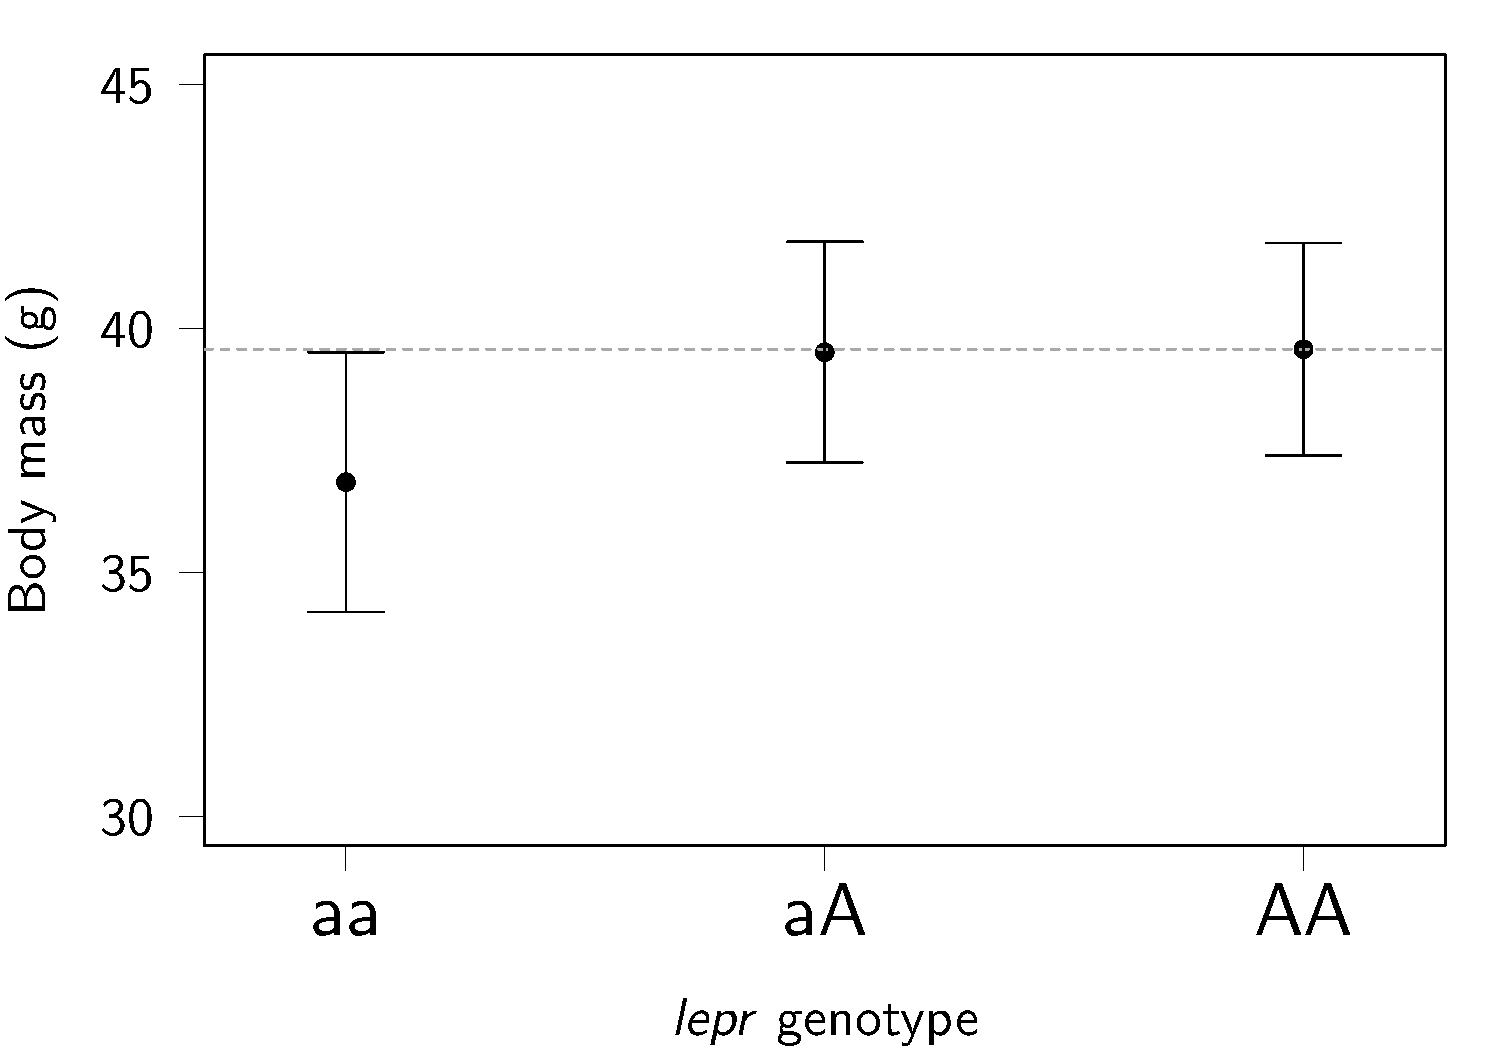
\includegraphics[width=0.5\textwidth]{FiguresGeneral/PhenoEffect-1}
	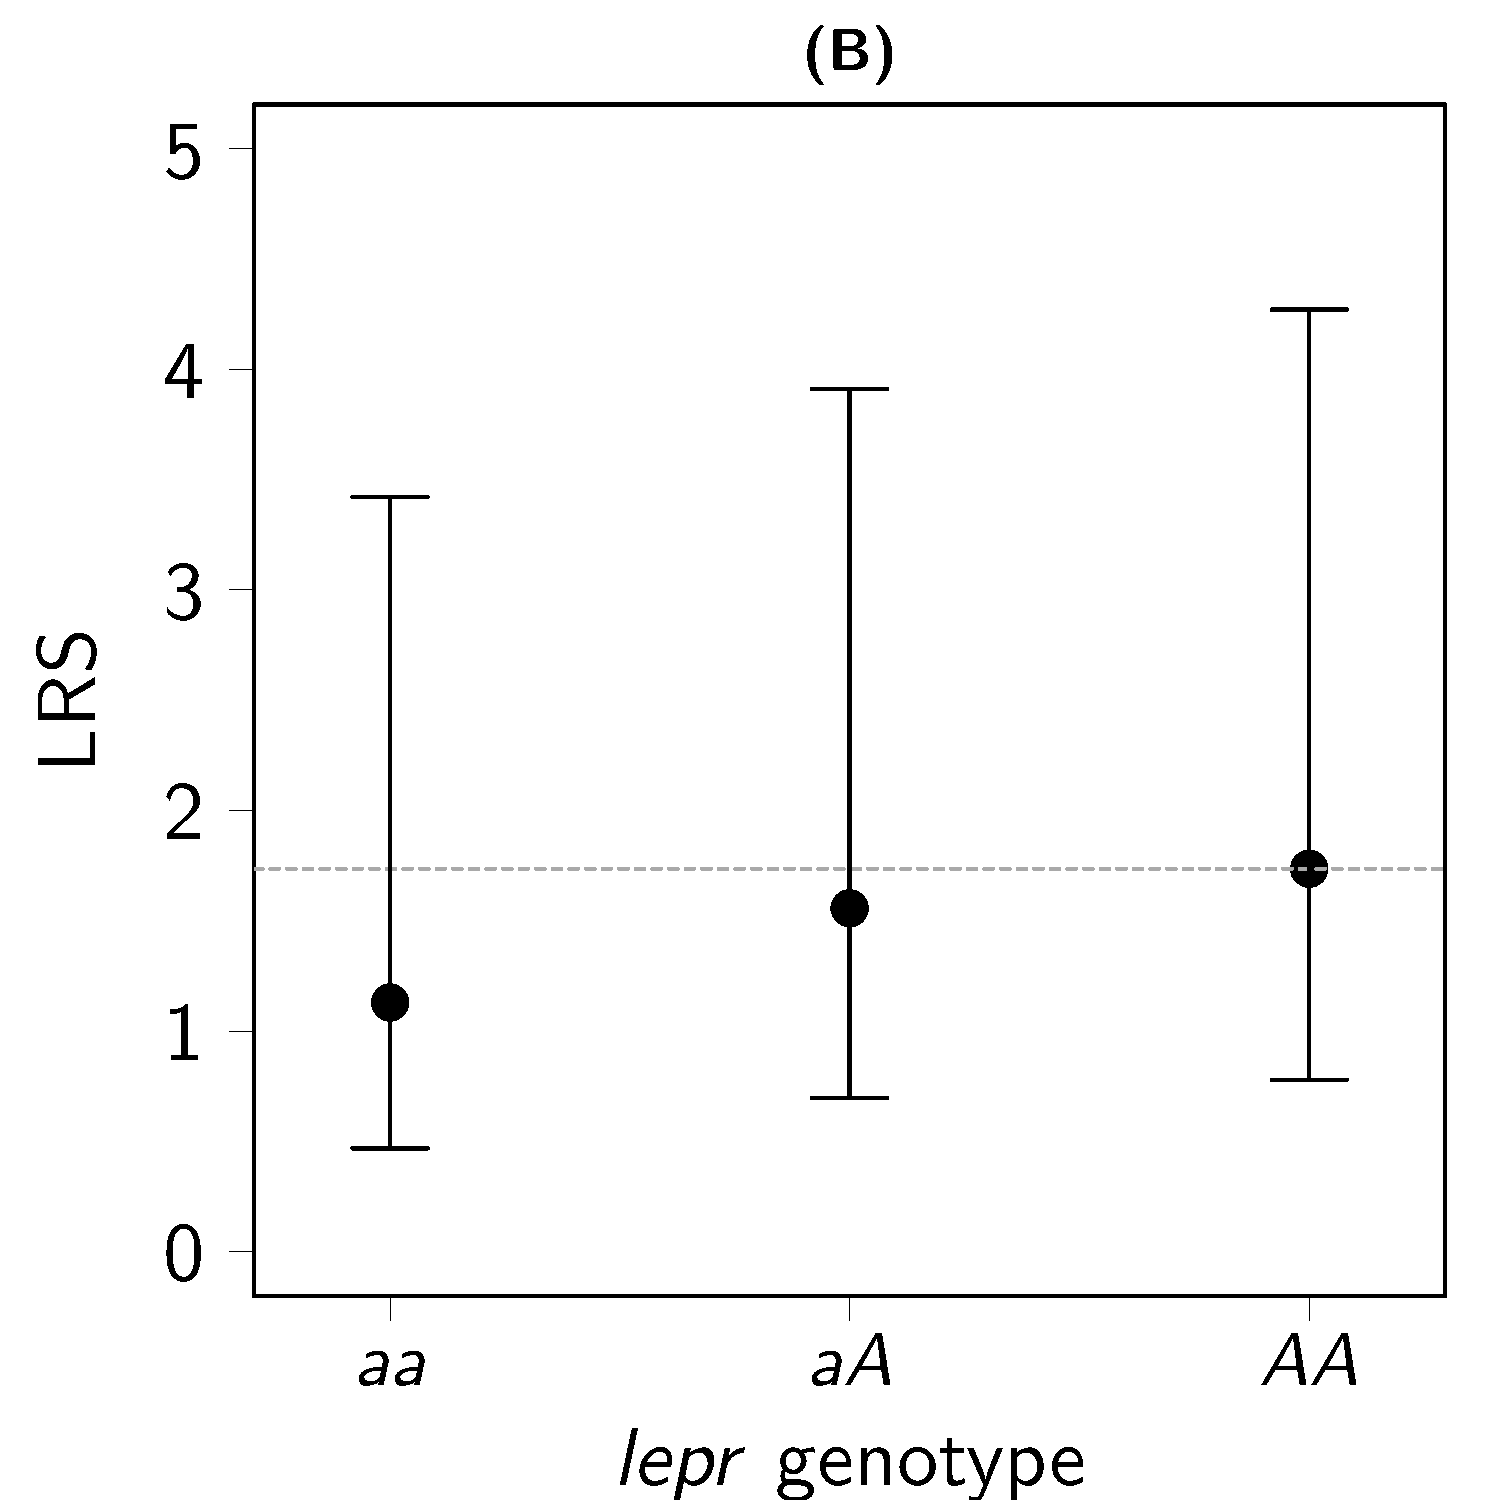
\includegraphics[width=0.5\textwidth]{FiguresGeneral/FitnessEffect-1}
	\caption{Body mass and lifetime reproductive success (LRS) as a function of \emph{lepr} genotype. 
	(\textbf{A}) Expected body mass of snow voles bearing one of the three \emph{lepr} genotypes. The expectations and 95\% confidence intervals were predicted from a linear mixed model fitted to the 2311 mass measurements of 532 snow voles. The model accounted for sex, age, date of capture and their two-ways interactions, as well as year of capture and multiple measurements of the same individual.
	(\textbf{B}) Expected LRS of snow voles bearing one of the three \emph{lepr} genotypes. The expectations and 95\% confidence intervals were predicted from a Poisson generalized linear mixed model fitted to the lifetime reproductive success of 611 snow voles. The model accounted for inbreeding coefficient, year of birth and over-dispersion (using an observation-level random effect). For both panels, the dashed horizontal line projects the expected value of genotype \emph{AA} to ease comparison with \emph{Aa} and \emph{aa}.}
	\label{fig:leprpheno}
\end{figure}

Knowledge of both the effect of the three genotypes and the allele frequencies one can analytically compute the additive genetic variances associated with a bi-allelic locus \parencite[][p77]{Fisher1941average,Lynch1998}. The additive genetic variances associated with \emph{lepr} are $0.052 \text{g}^2$ for body mass and $0.006 \text{pup}^2$ for lifetime reproductive success. This means that for both traits, \emph{lepr} explains about 1\% of the additive genetic variation as estimated from an animal model. This is rather large for a single locus, as those studies that have a large enough sample size to avoid biases introduced by the Beavis effect, typically find that quantitative trait loci explain a fraction of a percent to a few percent of the additive genetic variance (V$_\text{A}$) \parencite{Flint2009,Jensen2014}. Nevertheless, 1\% of V$_\text{A}$ is not sufficient to infer the evolutionary potential of the trait, and genotyping many more markers, for instance using high-throughput sequencing \parencite{Goodwin2016}, is unlikely to improve this situation in this small population. Generally speaking, very large sample sizes and high-quality genomic resources are necessary to explain a biologically relevant proportion of the additive genetic variance \parencite{Bloom2013, Jensen2014}. For instance, 183,727 individuals were necessary to find 180 QTL that jointly explained only 13\% of additive genetic variation in human body height \parencite{LangoAllen2010}. Admittedly, high-throughput sequencing data can also been used in a top-down way, which does not aim to identify causal genetic variants, but instead quantifies the phenotypic variation jointly explained by all the genotyped markers. Using this approach, 3,925 individuals genotyped for 294,831 markers, \parencite{Yang2010} were able to explain 45\% of the genetic variation in human height. Albeit much better, provided knowledge on the relatedness among individuals is available, quantitative genetics can estimate all the additive genetic variance, and this without any genotyping effort.

To conclude, bottom-up approaches allow unravelling the molecular mechanisms underlying phenotypic variation. By opening the black box and revealing these mechanisms, they can identify where this variation comes from, how it is linked to the environment and what the target of natural selection is \parencite{DeJong2014}. Moreover, they contribute to building a genotype-phenotype map, a long-lasting challenge in evolutionary biology \parencite{Kirschner2010}.
In contrast, quantitative genetics lumps all the effects of individual genes and their interactions into a few parameters which are largely non-informative with respect to the underlying genetic architecture \parencite{Mackay2001,Nietlisbach2015,Huang041434}. However, quantitative genetics provides a simple and direct measure of key evolutionary parameters. As they are based directly on data on the phenotype, which is the target of selection and the source of ecological interactions, they provide simple measures of genetic parameters that can directly be interpreted within the ecology of organisms.
This thesis is concerned with the genetics and evolution at the level of organisms, in relation to their environment, and accordingly, most of my work relies on quantitative genetics.

%%%%%%%%%%%%%%%%%%%%%%%%%%%%%%%%%%%%%%%%%%%
\section{This thesis}
\subsection{Objectives}
In this thesis, I investigate the causes of individual-level variation in fitness, and the consequences of this variation at the population level. This thesis aims at improving the measurement, and thereby our understanding, of selection and evolution in the wild. It examines the relative importance of stochasticity and selection in shaping reproductive success and survival, disentangles evolutionary from plastic changes, and explores the link between selection and evolution. These questions are addressed using a combination of computer simulations and data from the long-term individual-based monitoring of a snow vole population.

\subsection{Snow voles in Churwalden}
% Species
The snow vole (\textit{Chionomys nivalis}, Martins 1842) is a medium-sized rodent, its adult body size ranges from 10 to 14 cm, without the tail (5 to 7.5 cm long). Contrary to the widespread idea that snow voles are white, the fur colour of the upper-parts varies from light to dark taupe grey, sometimes tinted with brown or dark red (Fig. \ref{fig:juvvole}). Indeed, the species could probably be renamed \emph{rock vole}: it is a rock, rather than a snow, specialist \parencite{Luque-larena2002} and might be associated with high elevations and snow only because rocky areas are more widespread there. It is sparsely distributed across southern Europe and Asia Minor, from sea level up to 4000 m of elevation \parencite{Janeau1997}.
\begin{figure}[ht]
	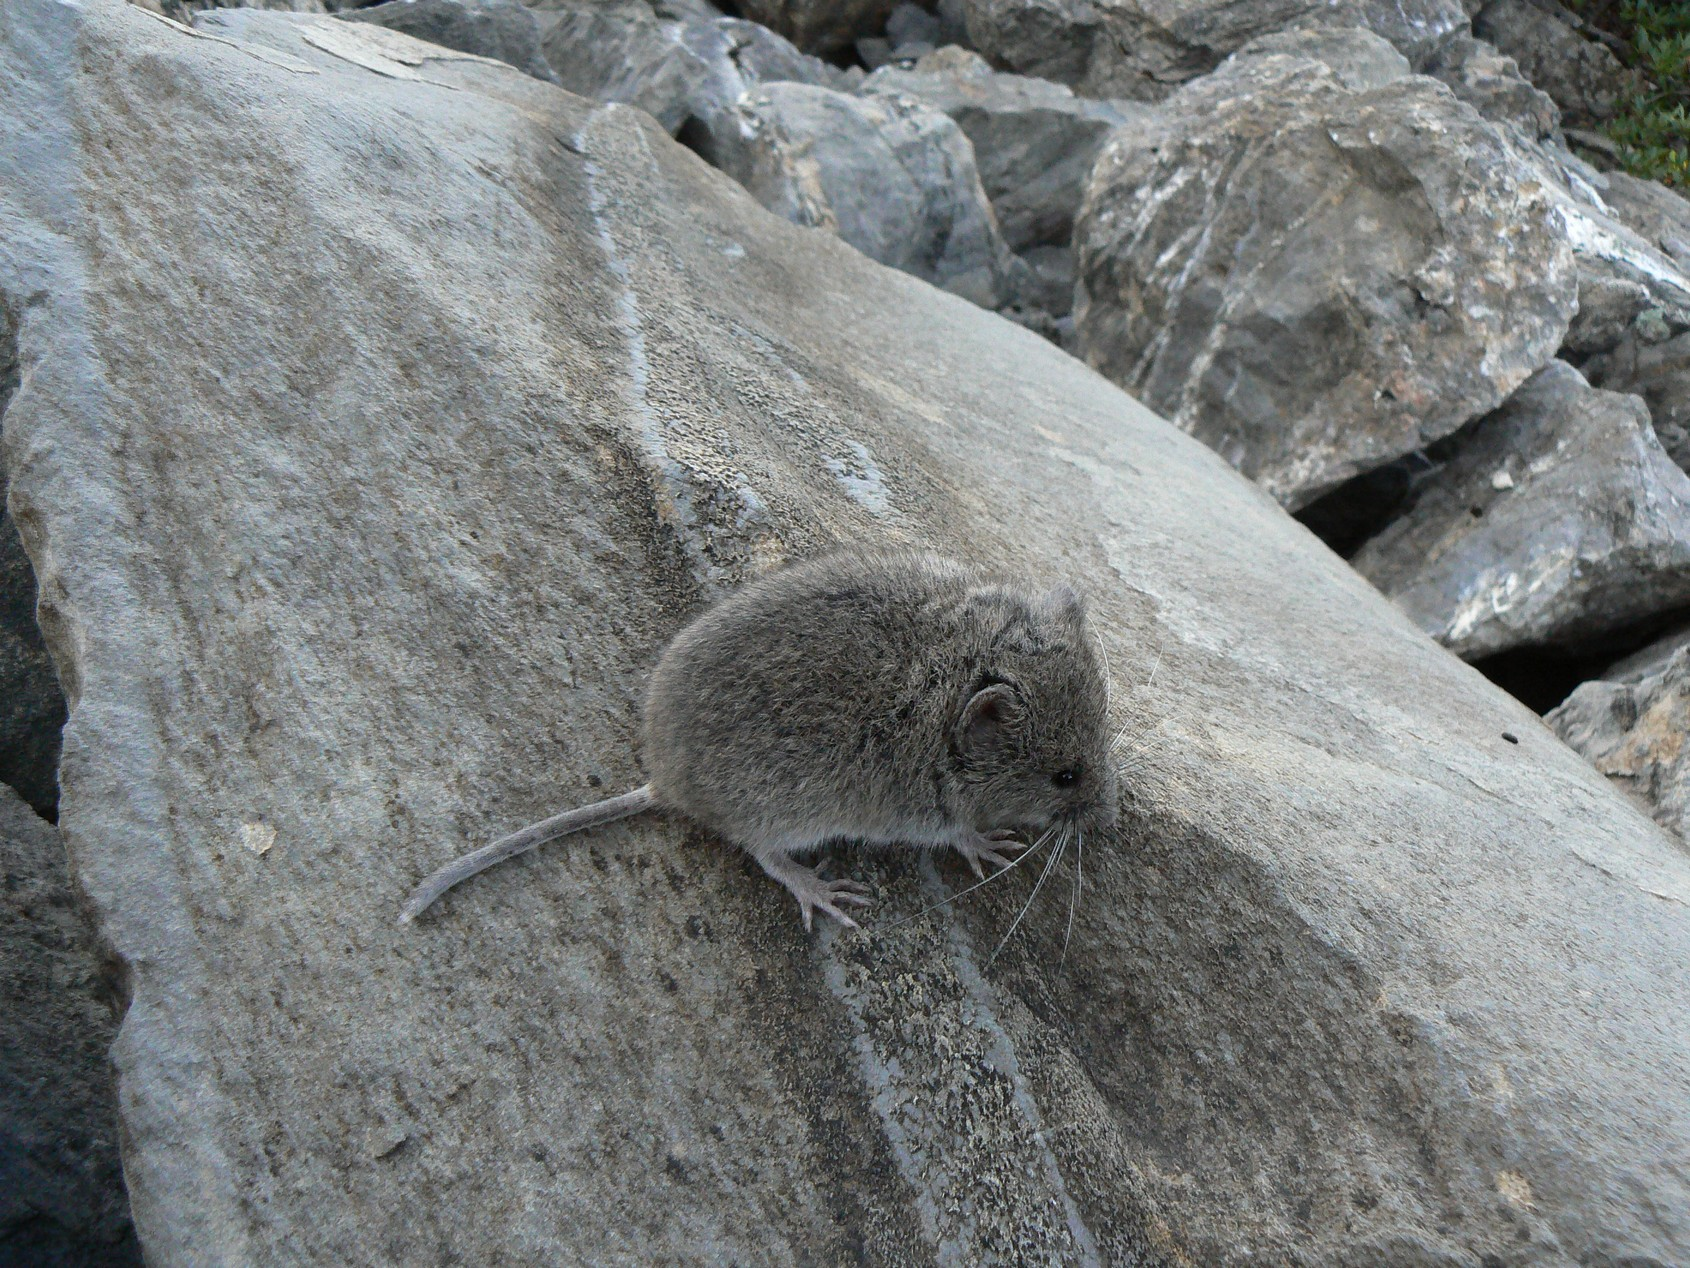
\includegraphics[width=0.49\textwidth]{FiguresGeneral/juvvole.JPG}
	\hspace{0.02\textwidth}
	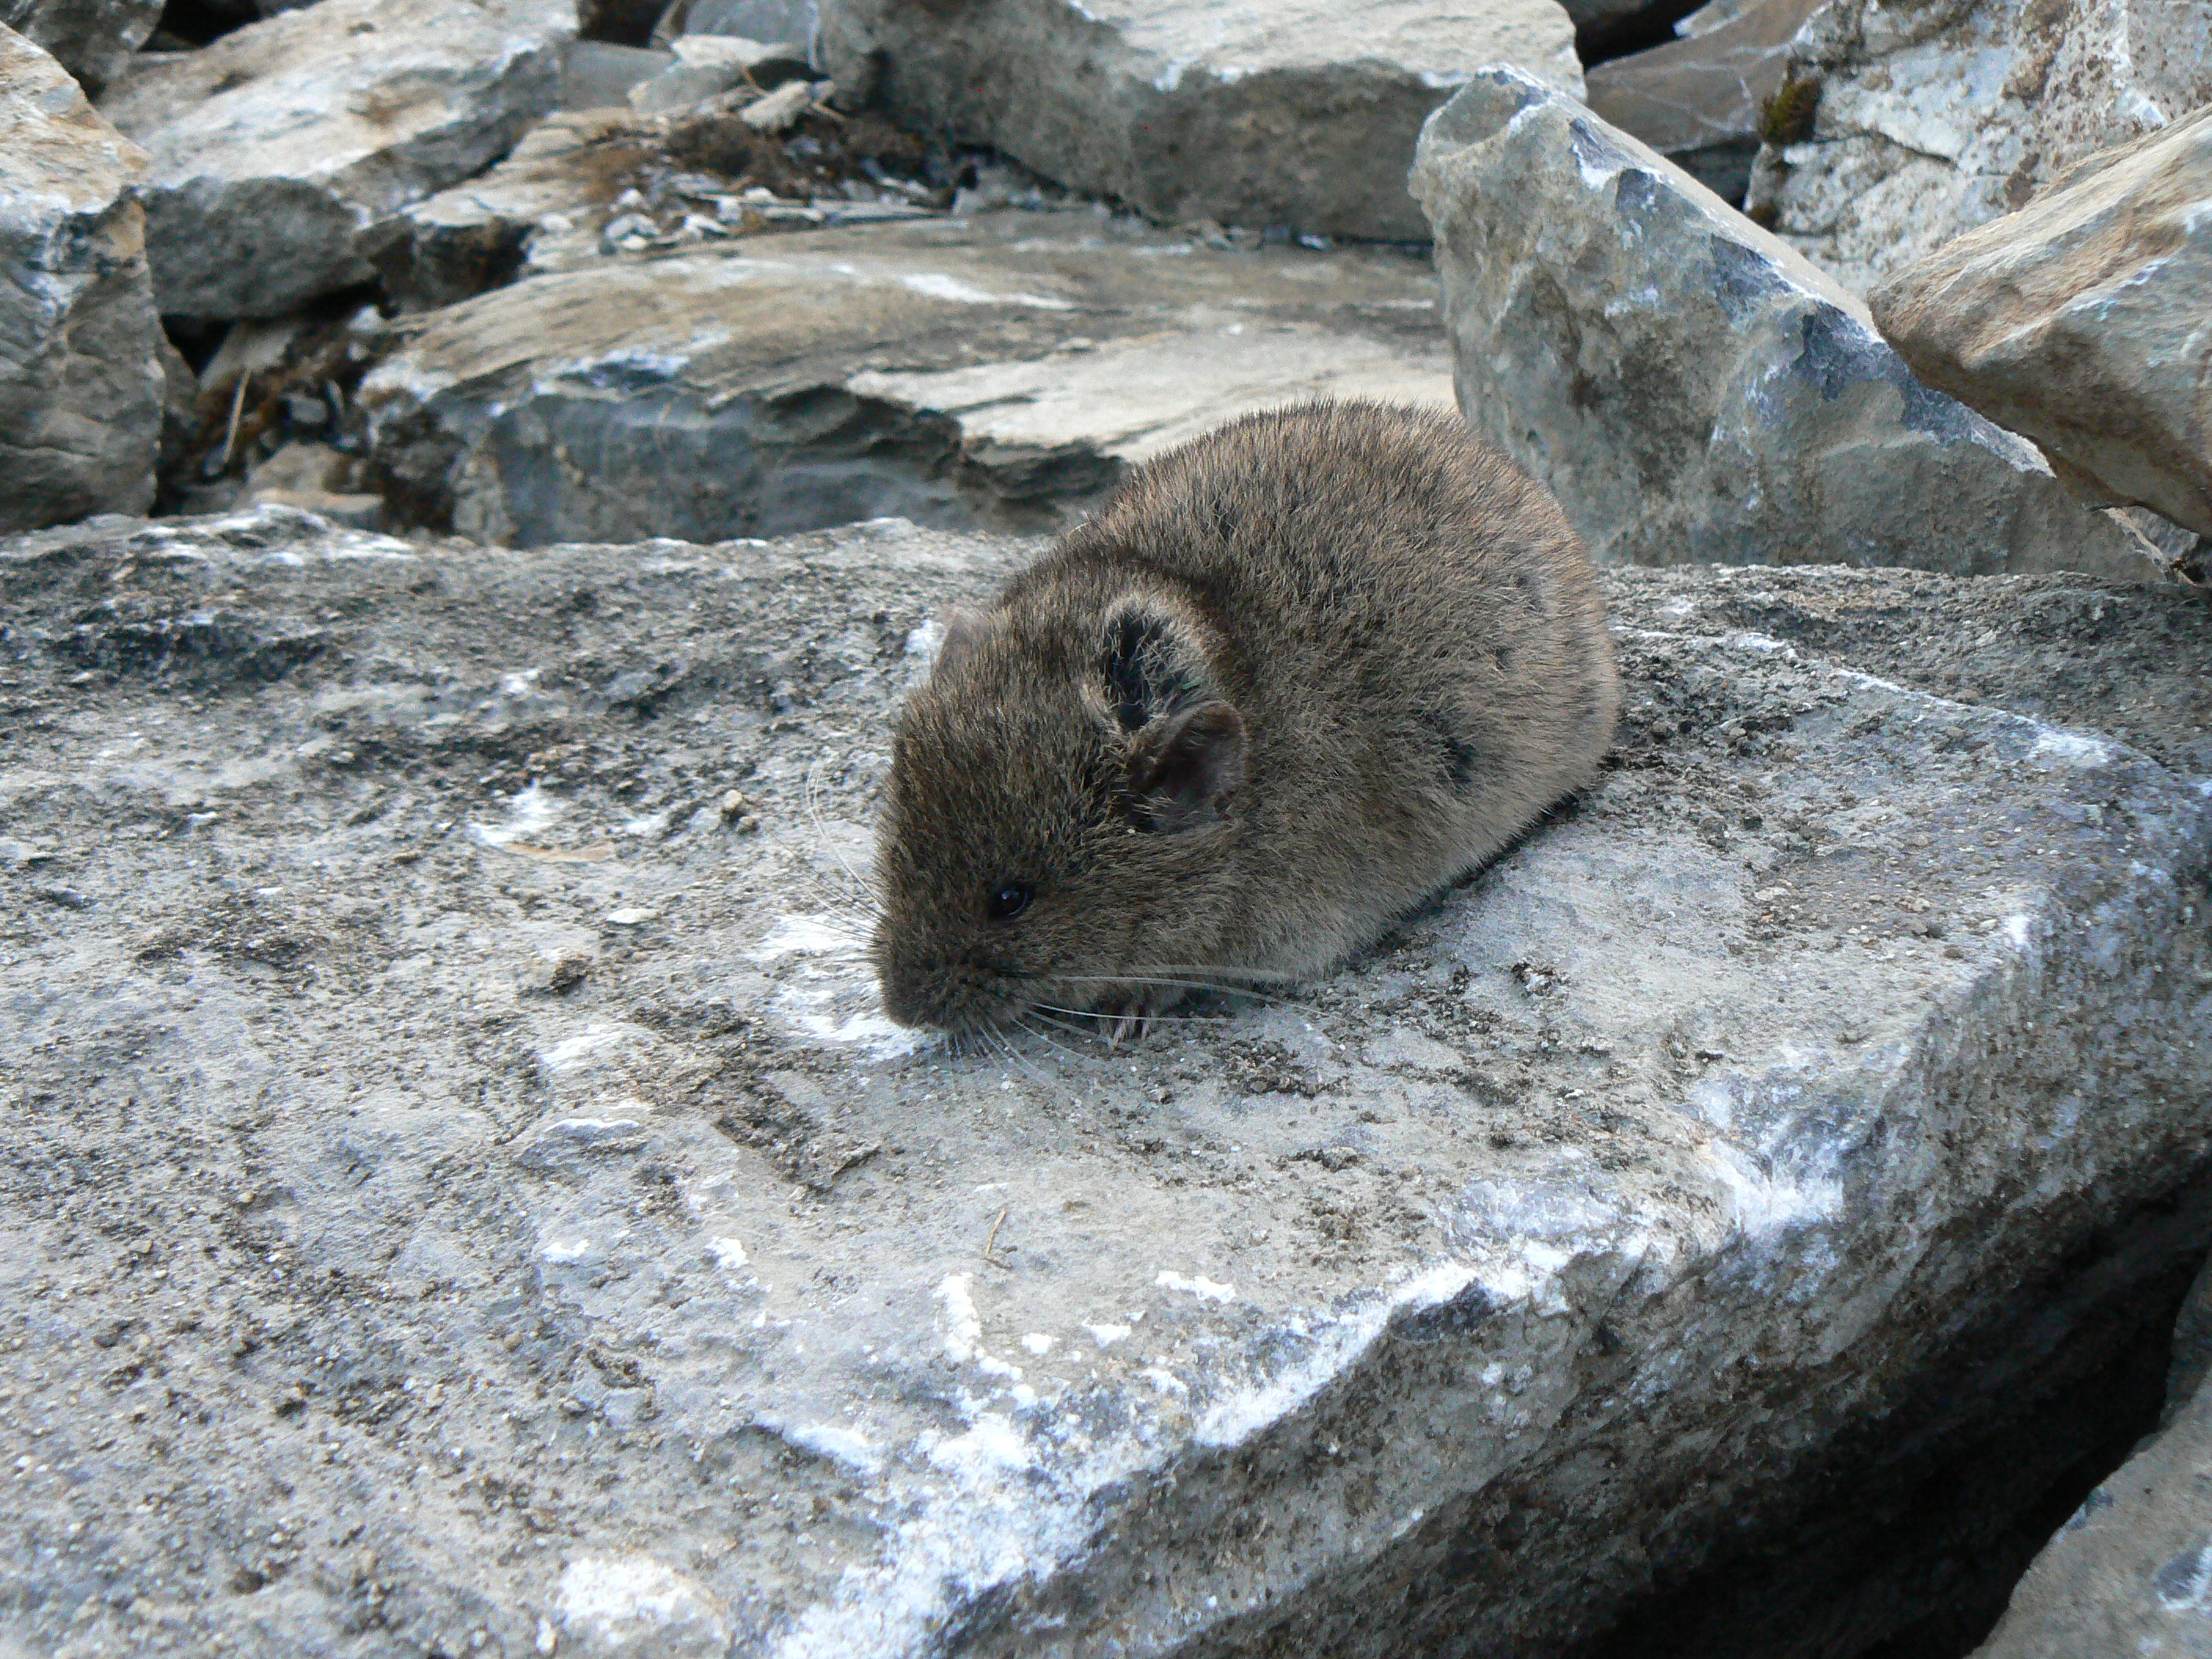
\includegraphics[width=0.49\textwidth]{FiguresGeneral/advole.JPG}
	\caption{Juvenile (left picture) and adult (right picture) snow voles in their habitat in Churwalden, Switzerland. Juveniles always lack the brown hue generally found in adults. Neither adults nor juveniles are white.}
	\label{fig:juvvole}
\end{figure}

Snow voles excavate burrows under the rocks, but can also use natural clefts between rocks, sometimes carrying small stones to build walls \parencite{Niederer2008}. A burrow consists of tunnels connecting chambers, one for the nest and multiple ones to stock dry plants \parencite{Janeau1997}. The species is not known to hibernate or migrate and is therefore exposed to harsh winter conditions in its high-elevation range. 
Adult females actively defend small territories against non-relatives, and tend to form matrilineal clusters of territories, whereas adult males wander and fight across large overlapping home-ranges \parencite{Luque-larena2004, Garcia-Navas2016}. The matting system is promiscuous and a same litter can be sired by multiple males. Females normally produce 1 to 4 litters of 1 to 5 pups between May and September. Juveniles generally do not reproduce in their first civil year. 
Although they can eat flour worms in the lab, there is no evidence that snow voles are not strictly herbivorous in the wild \parencite{Janeau1997}. In the Swiss Alps, snow voles suffer predation from red foxes, stoats, various owls and corvids, and parasitism from flees, lices and ticks \parencite{Janeau1997, Martinoli2001}.

% Population, characteristics
The study area is located near the Churer Joch, Churwalden, in the Swiss canton Graub\"unden (Fig. \ref{fig:map}; coordinates $46^{\circ}$48' N, $9^{\circ}$34' E), and covers about 5 ha between 1980 m and 2100 m above sea level. It consist of a west-exposed scree interspersed with small coniferous trees and with patches of alpine meadow. The study area is demarcated by extensive meadows to the south and to the north, by a coniferous forest to the west and by cliff to the east (Fig. \ref{fig:landscape}). 
\begin{figure}[ht]
	\centering
	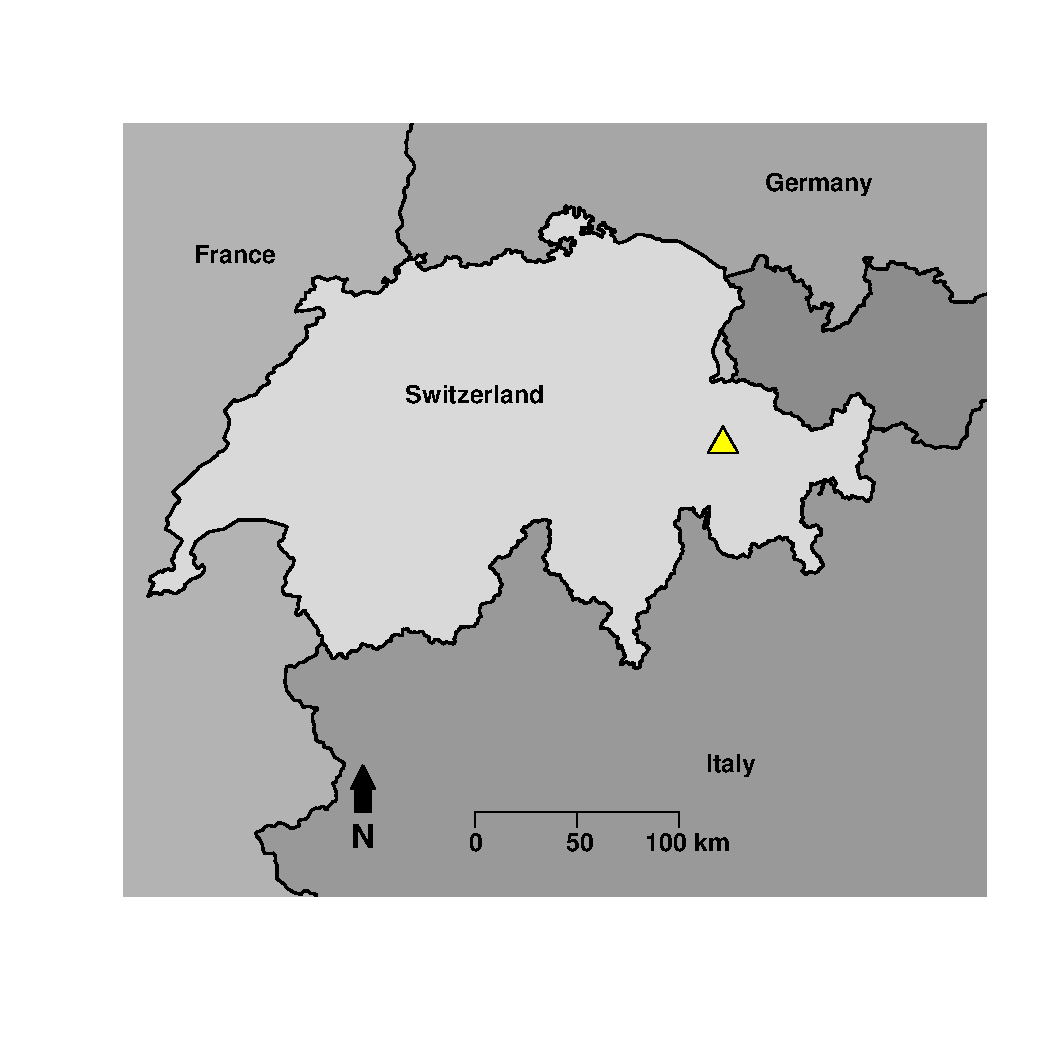
\includegraphics[width=0.6\textwidth]{FiguresGeneral/Map/figure/map-1.pdf}
	\caption{Location of the study area in Switzerland. The yellow triangle indicates the study area, with coordinates $46^{\circ}$48' N, $9^{\circ}$34' E, by Churwalden, in the Swiss canton Graub\"unden. Countries are filled with different shades of grey, Austria and Lichtenstein are not labelled.}
	\label{fig:map}
\end{figure}

\begin{figure}[ht]
	\includegraphics[width=1\textwidth]{FiguresGeneral/DSC_2111viewontaliflue}
	\caption{Distant view of the field site, taken from the west. The trapped area covers about a fifth of the width and a tenth of the height of the picture and is located in the centre. This scree is surrounded by a forest, a cliff and meadows.}
	\label{fig:landscape}
\end{figure}
Another scree offers about 1 ha of favourable habitat, starting 300 m north-east to the monitored area. This area was trapped in 2008 and 2013. The snow vole density was rather low, with on average five captures per night of trapping, versus 18 on the main study area. More habitat favourable to snow voles can be found 2 Km to the south. The study population is moderately isolated and receives 5 to 10 immigrants per year, on a total of 60 to 180 individuals \parencite{Garcia-Navas2016}. 

% Monitoring and history
The monitoring of this snow vole population was initiated in 2006 by Dr. Peter W. Wandeler. Dr. Erik Postma took the monitoring over in 2012, but the protocol has remained practically unchanged. This thesis contains data collected up to the year 2015.
\begin{figure}[ht]
	\begin{tikzpicture}
		\node (pic) at (0,0) {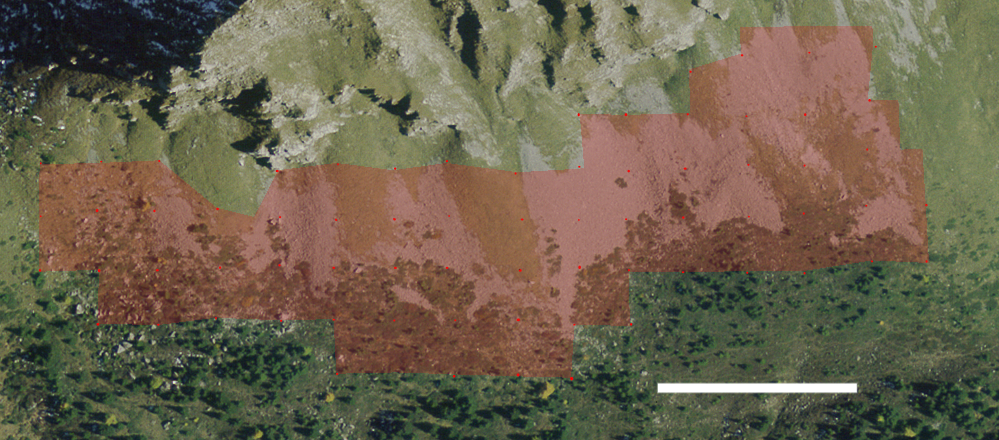
\includegraphics[width=1\textwidth]{FiguresGeneral/fieldposts2.PNG}};
		\draw[<-, ultra thick, color=white,>=stealth] (6.5,-2.5)--(7.5,-2.65);
		\node (n) at (6.3,-2.4) {\color{white}{N}};
		\draw[ultra thick, color=black] (2.52,-2.59)--(2.52,-2.75)--(5.68,-2.75)--(5.68,-2.59);
		\node (m) at (4.1,-3) {\color{white}{100 m}};
		%\draw[ultra thick, color=black] (2.52,-2.75)--(2.52,-2.65);
		%\draw[ultra thick, color=black] (5.68,-2.75)--(5.68,-2.65);
	\end{tikzpicture}
	\caption{Orthophoto of the study site, from 2008. The red shading indicates the approximate area where traps are set.}
	\label{fig:fieldarea}
\end{figure}
Every year from 2006 to 2016, snow voles were life-trapped multiple times between late May and early October. Traps were set during the day, opened around sunset and checked the next morning. 
For every snow vole capture \footnote{Other species (bank voles, pine voles, wood mice, stoats, black salamanders, slugs\dots) were released without taking measurements.}, we recorded sex, age, body mass, body length, tail length, date, location and signs of reproductive activity (pregnancy, lactation, swollen scrotum). 
In addition, all newly-captured snow voles were individually marked and genotyped for 18 microsatellites \parencite{Wandeler2008}. Based on the autosomal microsatellite genotypes, we reconstruct the pedigree of the population. This pedigree is the raw material for most of the work presented in this thesis. In particular, it is used to define reproductive success, as well as to estimate the relatedness between all pairs of individuals. These two statistics are essential to estimate selection, fitness and genetic variation. 


\subsection{Thesis outline}
In natural populations, fitness is generally measured using individual measures of reproductive success and survival. Importantly, these are proxies of fitness and their variation has a large stochastic component. This has lead some authors to doubt that there is any significant variation in fitness in natural populations. Recent methodological developments appeared to support the view that variation in reproduction and survival was purely stochastic, and suggested that the potential for selection and evolution in the wild was strongly overestimated. In \textbf{chapter \ref{chap:dynhet}} I examine these methods and, based on computer simulations, demonstrate that they lack the statistical power to detect latent variation in fitness components. Using an alternative approach I show the presence of significant variation in the propensity of reproductive success in the snow vole population, thereby showing some potential for selection and adaptive evolution in this population. I also attempt to clarify some conceptual misunderstandings between the proponents of the two methodological schools. 

In \textbf{chapter \ref{chap:decpop}}, with collaborators from different methodological schools, I review and compare four frameworks that claim to be able to disentangle the causes of temporal phenotypic change. While these frameworks appear to come to different conclusions with respect to the relative roles of plasticity, demography and genetic change, based on computer simulations and mathematical comparisons, we show that these discrepancies primarily originate from different definitions of the components of change. Nevertheless, one of these frameworks, the quantitative genetics \emph{animal model}, stands out as the only framework able to estimate genetic change and the response to selection (that is, the trans-generational consequence of variation in fitness). I relied heavily on this framework for the two next chapters.  

In \textbf{chapter \ref{chap:stasis}}, I explore the reasons of the mismatch between apparent phenotypic selection, phenotypic change and genetic change for body mass. I describe one of the first cases of contemporary adaptive evolution of a quantitative trait in the wild. Both the evolution and the selective pressure responsible for it are invisible to purely phenotypic approaches, however. Using multivariate animal models, I identify the main component of selection as juvenile viability. I then infer that the target of selection is potential adult mass in juveniles and that selection is related to a recent change in climatic conditions. 

The previous chapter considered selection and evolution averaged over the whole study period, without considering their temporal dynamics across the study period. Fluctuating selection is thought to be a major determinant of the rate of evolution, and a potentially important process when it comes to understanding adaptation in the wild. 
Nevertheless, unbiased measures of the variation of selection are rare, and the coupling between variation in selection and variation in evolution has been largely ignored. \textbf{Chapter \ref{chap:flusel}} shows that selection fluctuates in the snow vole study population, mainly due to variation in fertility selection. The rate of adaptive evolution is, however, remarkably constant, because viability selection, the driver of body mass evolution, does not vary. In this case the fluctuation of selection is evolutionary irrelevant. These two last chapters highlight the dangers of relying on phenotypic estimates of selection to understand the evolutionary dynamics of natural populations.

Finally, in \textbf{chapter \ref{chap:discu}}, I summarize the progresses made during this Ph.D. on the understanding of natural populations, and discuss some of the remaining challenges and future directions.

%\printbibliography[heading=subbibliography]